\begin{exercise}
Betrachten Sie das System
\begin{align*}
  x^{\prime} &= -x(x - a)(x - b) - y \\
  y^{\prime} &= \sigma x - \gamma y,
\end{align*}
wobei $0 < a < b$ und $\sigma, \gamma > 0$.
\begin{enumerate}[label = \textbf{\alph*)}]
\item Bestimmen Sie die Ruhelagen des Systems. Skizzieren Sie das Phasenportrait,
also deuten Sie durch Pfeile das Richtungsfeld (Vektorfeld $\bf{f(y)}$ der
autonomen ODE $\bf{y^{\prime} = f(y)}$) an.
\item Ist die Ruhelage $(0,0)$ asymptotisch stabil?
\item Geben Sie die Differentialgleichung an, die von der Ableitung der Lösung
nach $\sigma$ erfüllt wird.
\end{enumerate}
\end{exercise}
\begin{solution}
  \FloatBarrier
  \begin{figure}
      \centering
      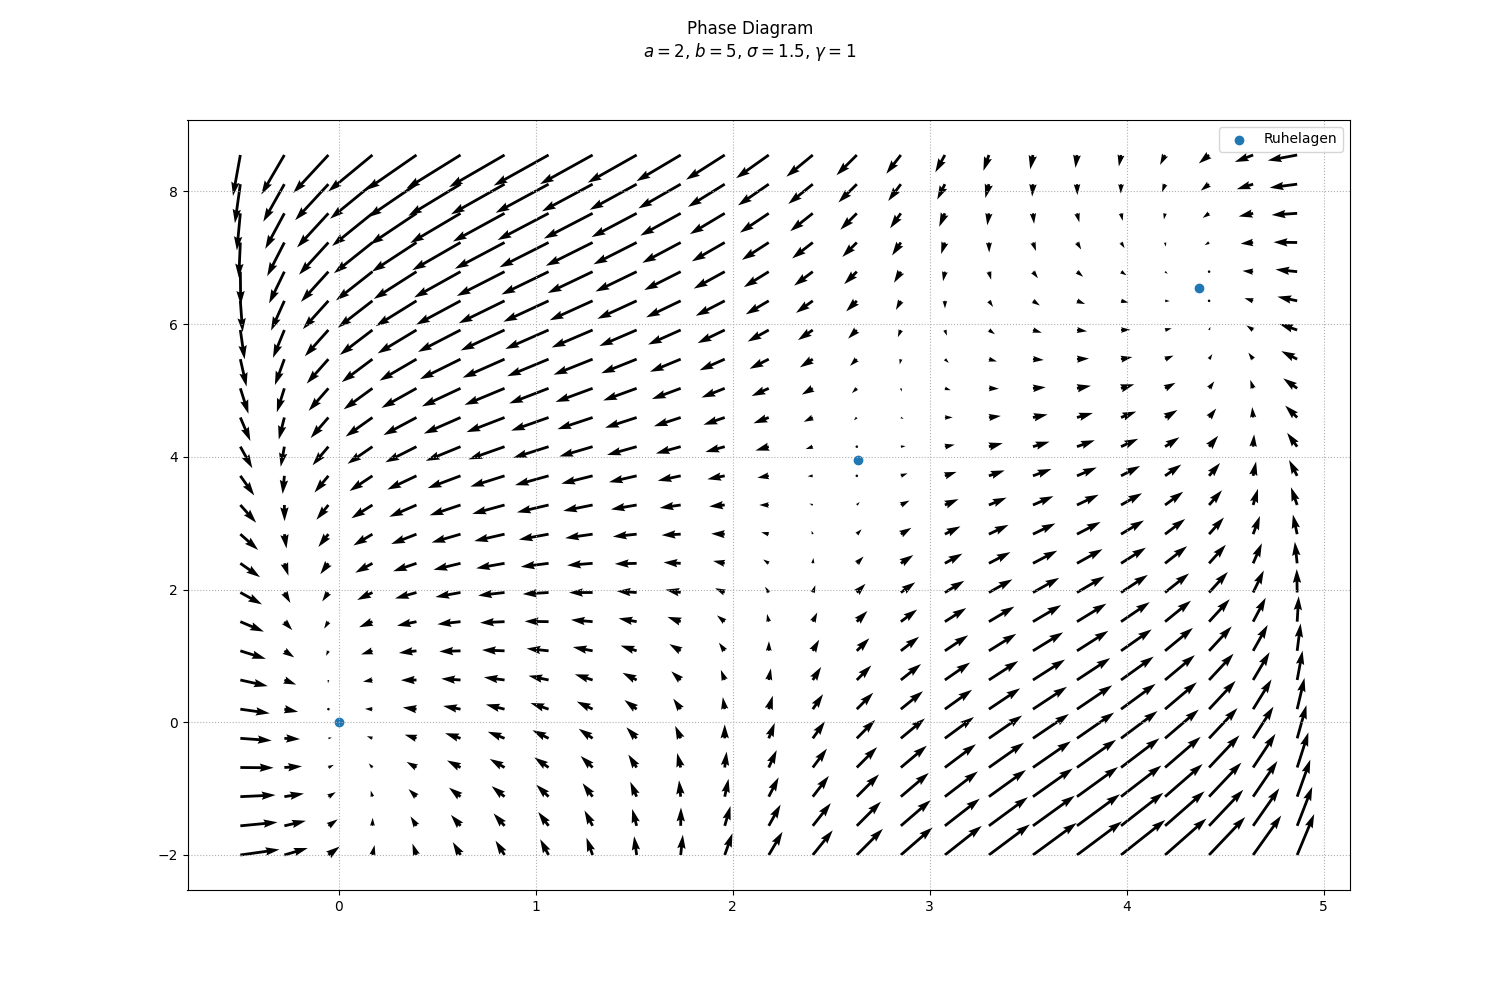
\includegraphics[width=\linewidth]{plot7-2.png}
  \end{figure}
  \FloatBarrier
\leavevmode \\
\begin{enumerate}[label = \textbf{\alph*)}]
\item Um die Ruhelagen zu bestimmen setzen wir einfach die Differentialgleichung
\begin{align*}
  f\left(\begin{pmatrix}
    x \\ y
  \end{pmatrix}\right) =
  \begin{pmatrix}
    -x(x - a)(x - b) - y \\
    \sigma x - \gamma y
  \end{pmatrix}
  = \begin{pmatrix}
    0 \\ 0
  \end{pmatrix}.
\end{align*}
Leicht erkennt man, dass $(0,0)^{\top}$ eine Ruhelage darstellt.
Für $(x,y)^{\top} \neq (0,0)^{\top}$ erhalten wir aus der zweiten Zeile
\begin{align*}
   \frac{\sigma}{\gamma}x =  y.
\end{align*}
Setzen wir das in die erste Zeile ein, erhalten wir
\begin{align*}
  -x(x - a)(x - b) - \frac{\sigma}{\gamma}x &\stackrel{!}{=} 0 \\
  \iff (x - a)(x - b) + \frac{\sigma}{\gamma} &\stackrel{!}{=} 0 \\
  \iff x^2 -(a+b)x + ab + \frac{\sigma}{\gamma} &\stackrel{!}{=} 0 \\
  \iff x &= \frac{a+b}{2} \pm \sqrt{\frac{(a+b)^2}{4} - ab - \frac{\sigma}{\gamma}} \\
  \iff x &= \frac{a+b}{2} \pm \sqrt{\frac{(a-b)^2}{4}  - \frac{\sigma}{\gamma}}.
\end{align*}
und mit
\begin{align*}
  y = \frac{\sigma}{\gamma}\left(\frac{a+b}{2} \pm \sqrt{\frac{(a-b)^2}{4} - \frac{\sigma}{\gamma}}\right)
\end{align*}
unsere letzten beiden Ruhelagen.
\item Zur Untersuchung der Stabilität von $(0,0)^{\top}$ verwenden wir das Prinzip
der linearisierten Stabilität. Dazu berechnen wir uns
\begin{align*}
Df((x,y)^{\top}) = \begin{pmatrix}
  -3x^2 + 2(a+b)x - ab & -1 \\
  \sigma & - \gamma
\end{pmatrix}
\end{align*}
und erhalten
\begin{align*}
  Df((0,0)^{\top}) =
  \begin{pmatrix}
    - ab & -1 \\
    \sigma & - \gamma
  \end{pmatrix}.
\end{align*}
Das charakteristische Polynom lautet
\begin{align*}
  \chi(\lambda) = (ab + \lambda)(\gamma + \lambda) + \sigma \stackrel{!}{=} 0
\end{align*}
mit den Nullstellen
\begin{align*}
  \lambda_{1,2} = -\frac{ab+\gamma}{2} \pm \sqrt{\frac{(ab + \gamma)^2}{4} -ab\gamma - \sigma}.
\end{align*}
Nun unterscheiden wir zwei Fälle:
\begin{itemize}
  \item $\frac{(ab + \gamma)^2}{4} -ab\gamma - \sigma < 0$: Dann ist
  \begin{align*}
    \Re\left(-\frac{ab+\gamma}{2} \pm \sqrt{\frac{(ab + \gamma)^2}{4} -ab\gamma - \sigma}\right)
    = -\frac{ab+\gamma}{2} < 0.
  \end{align*}
  \item $\frac{(ab + \gamma)^2}{4} -ab\gamma - \sigma > 0$: Da $ab\gamma, \sigma > 0$
  gilt
  \begin{align*}
    \Re\left(-\frac{ab+\gamma}{2} \pm \sqrt{\frac{(ab + \gamma)^2}{4} -ab\gamma - \sigma}\right)
    < \Re\left(-\frac{ab+\gamma}{2} \pm \sqrt{\frac{(ab + \gamma)^2}{4}}\right) \leq 0.
  \end{align*}
\end{itemize}
Mit Satz 5.8 ist $(0,0)^{\top}$ ist somit asymptotisch stabil.

\item ***Leichtere Version !?????!?? ***

Sei $z = \begin{pmatrix}
  x \\ y
\end{pmatrix}$ eine Lösung, dann gilt $z' = \begin{pmatrix}
  x' \\ y'
\end{pmatrix} = \begin{pmatrix}
  -x(x-a)(x-b)-y \\ \sigma x - \gamma y
\end{pmatrix}$ und somit für die Ableitung nach $\sigma$:
\begin{align*}
\frac{dz'}{d\sigma} = \begin{pmatrix}
  0 \\ x
\end{pmatrix}
\end{align*}
Also löst $\Phi = \frac{dz}{d\sigma}$ die Differentialgleichung
\begin{align*}
  \Phi' = \begin{pmatrix}
    0 \\ x
  \end{pmatrix}
\end{align*}

**********

Um die Differentialgleichung der Ableitung nach $\sigma$ zu bestimmen,
definieren wir uns ein geeignetes Hilfssystem ($z = (x,y)^{\top}$):
\begin{align*}
  Y(t) &:= \begin{pmatrix}
    z(t) \\ \sigma
  \end{pmatrix} \text{ löst }
  Y^{\prime} = f(t,z,\sigma), \qquad Y(t_0) =
  \begin{pmatrix}
    z_0 \\ \sigma_0
  \end{pmatrix} =: Y_0 \\
    f(t,z,\sigma) &= \begin{pmatrix}
      f(t,z,\sigma) \\ 0
  \end{pmatrix} \\
  v(t) &:= \partial_{Y_0} Y_{t_0,z_0}(t) =
  \begin{pmatrix}
    \partial_{z_0} z_{t_0,z_0} & \partial_{\sigma_0} z_{t_0,z_0} \\
    \partial_{z_0} \sigma_{t_0,z_0} & \partial_{\sigma_0} \sigma_{t_0,z_0}
  \end{pmatrix}
\end{align*}
Nach Satz 4.6. gilt nun
\begin{align*}
  v^{\prime}(t) = \partial_Y f(t,z_{t_0,z_0}(t), \sigma)v(t), \qquad v(t_0) = I,
\end{align*}
also
\begin{align*}
\begin{pmatrix}
  \partial_{z_0} z_{t_0,z_0} & \partial_{\sigma_0} z_{t_0,z_0} \\
  \partial_{z_0} \sigma_{t_0,z_0} & \partial_{\sigma_0} \sigma_{t_0,z_0}
\end{pmatrix}^{\prime}
=
\begin{pmatrix}
  \partial_{z} f(t,z_{t_0,z_0}, \sigma) & \partial_{\sigma} f(t,z_{t_0,z_0}, \sigma) \\
  0 & 0
\end{pmatrix}
\begin{pmatrix}
  \partial_{z_0} z_{t_0,z_0} & \partial_{\sigma_0} z_{t_0,z_0} \\
  \partial_{z_0} \sigma_{t_0,z_0} & \partial_{\sigma_0} \sigma_{t_0,z_0}
\end{pmatrix}
\end{align*}
und es folgt
\begin{align*}
  (\partial_{\sigma_0} z_{t_0,z_0})^{\prime} &= \partial_z f(t,z_{t_0,z_0},\sigma) \partial_{\sigma_0} z_{t_0,z_0}
  + \partial_{\sigma} f(t,z_{t_0,z_0},\sigma) \partial_{\sigma_0} \sigma_{t_0,z_0} \\
  (\partial_{\sigma_0} \sigma)^{\prime} &= 0
\end{align*}
Aus $(\partial_{\sigma_0} \sigma)^{\prime} = 0$ und $\partial_{\sigma_0}\sigma(t_0) = 1$
folgt $\partial_{\sigma_0} \sigma = 1$ und
\begin{align*}
  (\partial_{\sigma_0}z_{t_0,z_0})^{\prime} =
  \partial_z f(t,z_{t_0,z_0},\sigma)\partial_{\sigma_0} z_{t_0,z_0}
  + \partial_\sigma f(t,z_{t_0,z_0},\sigma).
\end{align*}
\end{enumerate}
\end{solution}
